% Cardiac arrest early warning pipeline: results annex (standalone)
% All tables and figures from the full manuscript (main.tex), extracted into a
% self contained document. Research prototype only: nothing here is clinical
% evidence. Style note: no hyphens or dashes anywhere in the prose.

\documentclass[11pt]{article}

\usepackage[utf8]{inputenc}
\usepackage[T1]{fontenc}
\usepackage{amsmath}
\usepackage{graphicx}
\usepackage{booktabs}
\usepackage{caption}
\usepackage[hidelinks]{hyperref}
\usepackage[a4paper,margin=1in]{geometry}

\graphicspath{{images/}}

\title{Cardiac Arrest Early Warning Pipeline: Results}
\author{[Author names to be added]}
\date{23 September 2026}

\begin{document}

\maketitle

\begin{center}
\small
Research prototype. All results are pipeline demonstrations, not clinical
validation. Confidence intervals are patient level bootstrap intervals. The
synthetic cohort is inflated by design (deterministic drift); the real data
test uses 20 Holter patients without photoplethysmogram, blood pressure or
vitals, so its role is to bound the electrocardiogram only regime.
\end{center}

\section{Synthetic validation}
The synthetic cohort has 60 patients with 28 arrest events. Baselines and the
temporal model on the patient level validation split:

\begin{table}[h]
\centering
\caption{Model performance on the patient level validation split (AUROC).}
\begin{tabular}{lccc}
\toprule
Model & 1 h & 6 h & 24 h \\
\midrule
Logistic regression & 1.000 & 0.954 & 0.689 \\
Gradient boosting & 0.998 & 0.993 & 0.911 \\
FEAN temporal model & 1.000 & 0.844 & 0.667 \\
\bottomrule
\end{tabular}
\end{table}

On the two held out replay patients (one case, one control):

\begin{table}[h]
\centering
\caption{Held out replay evaluation (patient level bootstrap CIs).}
\begin{tabular}{lcccc}
\toprule
Horizon & Positives & AUROC [95\% CI] & AUPRC & Brier \\
\midrule
1 h & 12 & 1.000 [1.000, 1.000] & 1.000 & 0.025 \\
6 h & 72 & 0.891 [0.825, 0.922] & 0.785 & 0.315 \\
24 h & 288 & 0.946 [0.944, 0.948] & 0.976 & 0.137 \\
\bottomrule
\end{tabular}
\end{table}

\begin{table}[h]
\centering
\caption{Alert level metrics on the held out replay patients.}
\begin{tabular}{lc}
\toprule
Metric & Value \\
\midrule
First true alert before arrest & 21.7 h \\
Lead time of true alerts (min, median, max) & 0.6, 11.2, 21.7 h \\
False alarms on the control patient & 5 in 24 h (4.9 per patient day) \\
PPV at sensitivity 0.8 (1 h, 6 h, 24 h) & 1.000, 0.307, 1.000 \\
Sensitivity at 1 alert per day (1 h, 6 h, 24 h) & 1.000, 1.000, 1.000 \\
Time averaged AUC across lead time bins & 0.890 \\
\bottomrule
\end{tabular}
\end{table}

\begin{table}[h]
\centering
\caption{Feature block ablations (validation AUROC, 20 epochs each).}
\begin{tabular}{lcccc}
\toprule
Variant & 1 h & 6 h & 24 h & Replay alerts (case, control) \\
\midrule
Full & 1.000 & 0.859 & 0.619 & 247, 1 \\
Vitals only & 1.000 & 0.755 & 0.555 & 38, 0 \\
Vitals plus engineered & 1.000 & 0.845 & 0.718 & 51, 0 \\
Vitals plus embeddings & 1.000 & 0.816 & 0.574 & 245, 0 \\
\bottomrule
\end{tabular}
\end{table}

Fusion variants on the same synthetic split (per modality projections plus
gated fusion, modality attention or static weights, with explicit presence
masks): 6 h validation AUROC is 0.830 for gated fusion, 0.738 for attention and
0.859 for static weights against 0.769 for the concatenation baseline. With the
photoplethysmogram removed at evaluation time, gated and weighted fusion stay
stable (0.867 and 0.841) while attention fusion degrades to 0.488.

\begin{figure}[h]
\centering
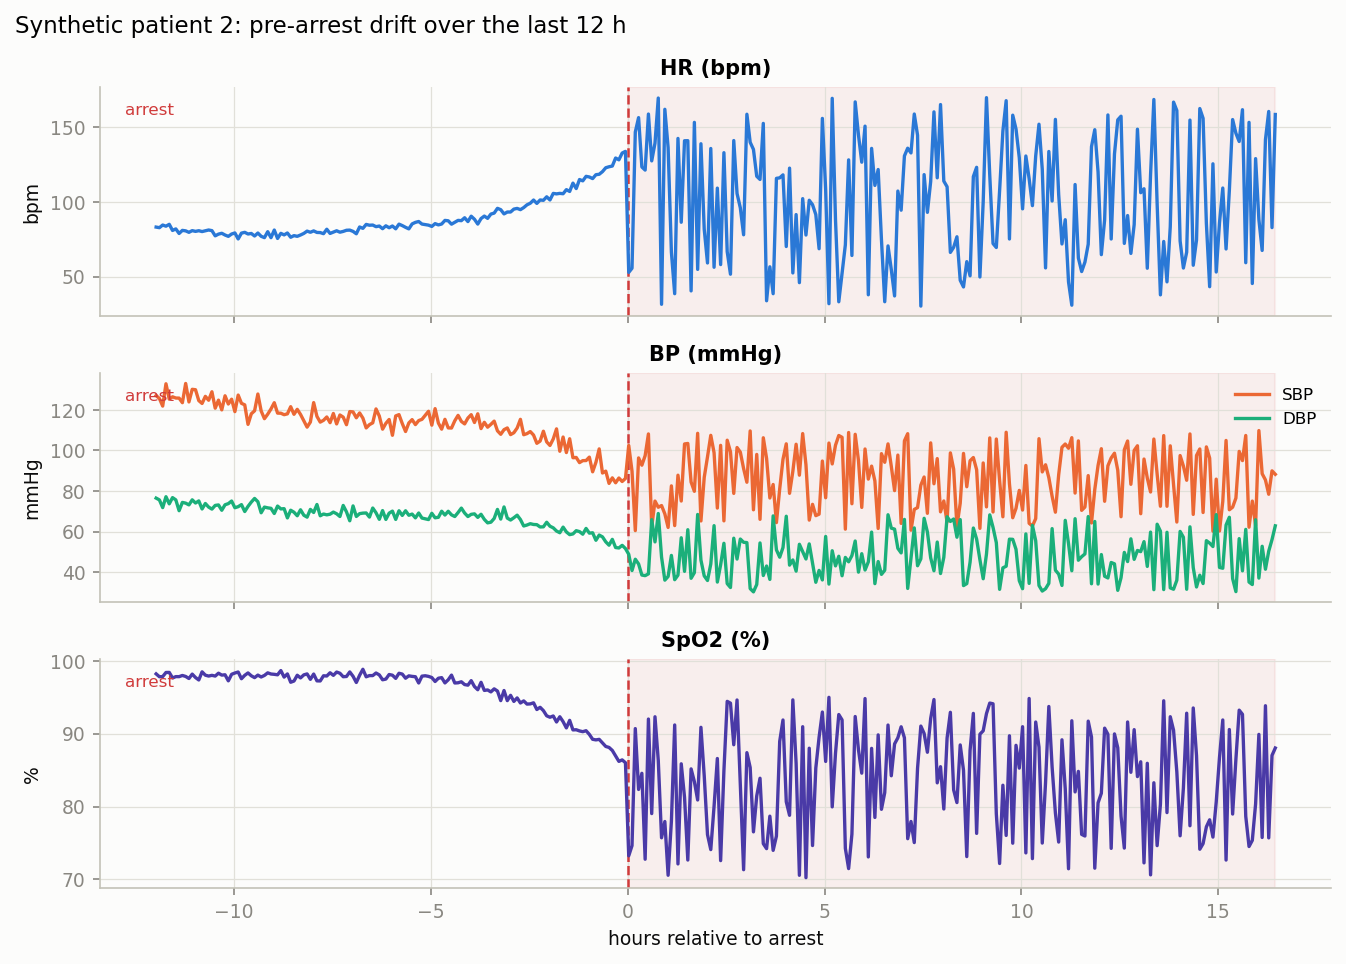
\includegraphics[width=\linewidth]{fig01_synthetic_drift.png}
\caption{Pre arrest drift of one synthetic case patient over the last 12 hours
before arrest (heart rate, blood pressure, saturation). The post arrest region
is shaded and excluded downstream.}
\end{figure}

\begin{figure}[h]
\centering
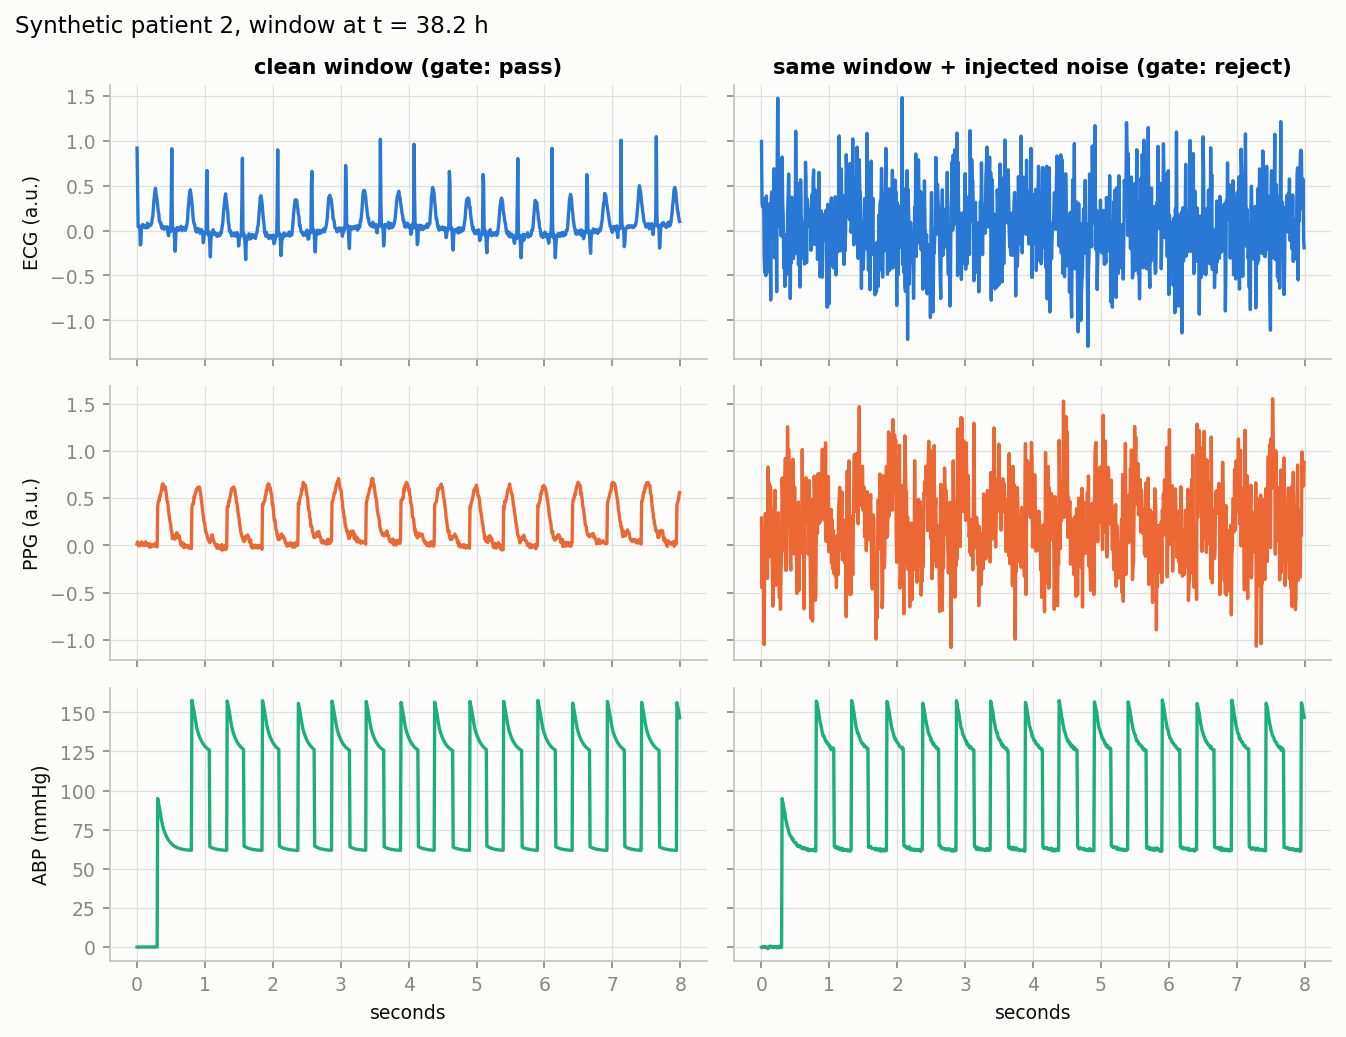
\includegraphics[width=\linewidth]{fig02_synthetic_waveforms.png}
\caption{One 30 second window: clean electrocardiogram, photoplethysmogram and
arterial pressure (left) versus the same window with an injected noise artifact
(right), which the quality gate rejects.}
\end{figure}

\begin{figure}[h]
\centering
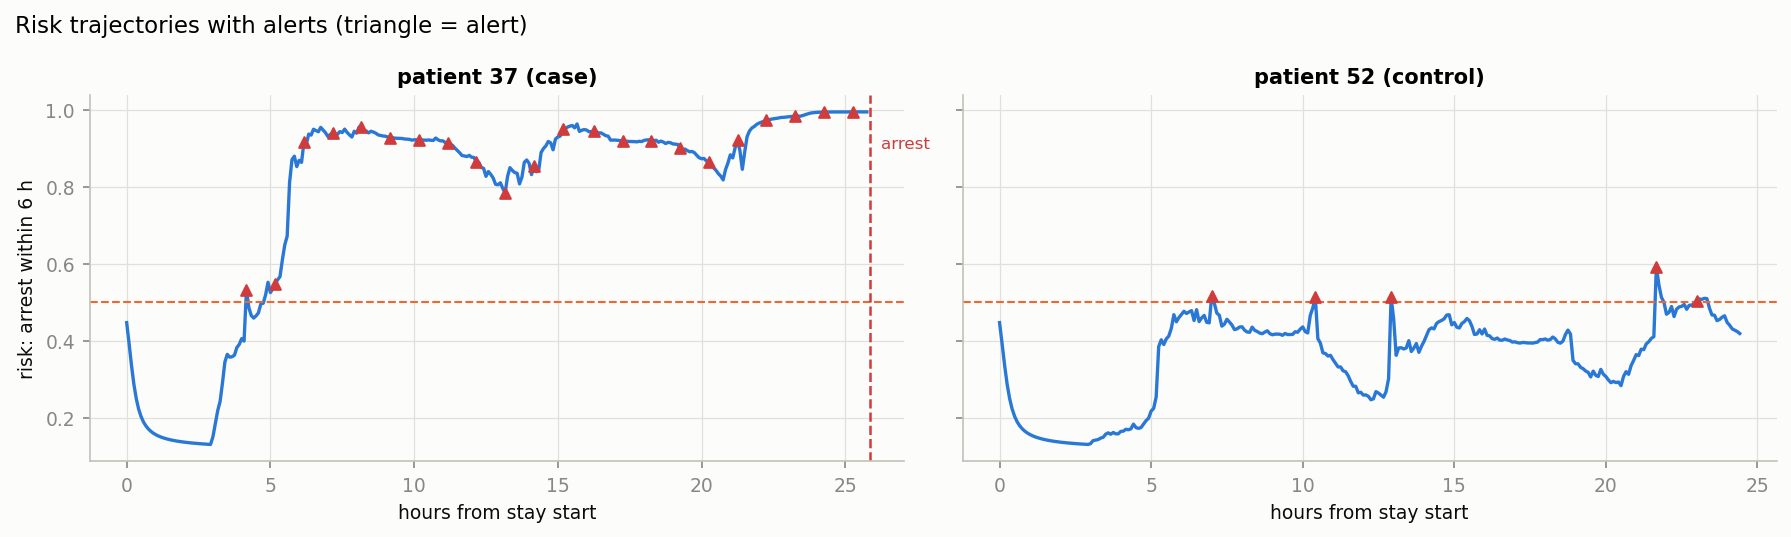
\includegraphics[width=\linewidth]{fig03_risk_trajectories.png}
\caption{Risk trajectories of the trained pipeline on the two held out
patients. Triangles mark alerts, the dashed line is the threshold. The case
patient (left) first crosses the threshold about 21 hours before arrest; the
control (right) produces a small number of false alarms.}
\end{figure}

\begin{figure}[h]
\centering
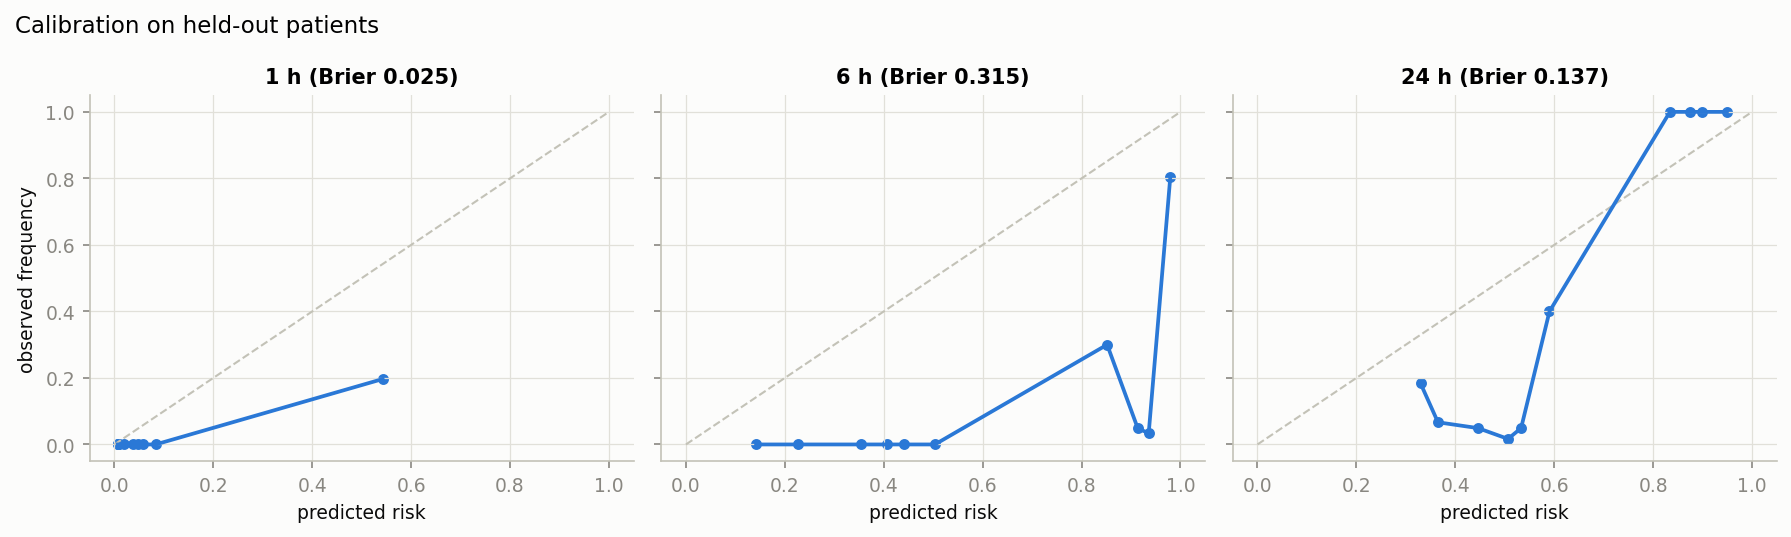
\includegraphics[width=\linewidth]{fig04_calibration.png}
\caption{Calibration curves per horizon on the held out patients. Predicted
risk versus observed frequency; the diagonal is perfect calibration.}
\end{figure}

\section{Real data stress test (Sudden Cardiac Death Holter Database)}
1829 real five minute windows from 20 records were embedded and evaluated with
a 5 fold cross validation grouped by patient. The 24 hour horizon is not
evaluable because no recording extends far enough before onset to supply 24
hour negatives. Sequence histories respect record and span boundaries and
seeds are fixed; confidence intervals are patient level bootstrap intervals.

\begin{table}[h]
\centering
\caption{Real data stress test (20 patients, 1829 windows).}
\begin{tabular}{lcc}
\toprule
Model & 1 h AUROC & 6 h AUROC \\
\midrule
Zero shot (synthetic trained model) & 0.338 & 0.447 \\
FEAN, concatenation (baseline) & 0.632 [0.516, 0.748] & 0.402 [0.344, 0.456] \\
FEAN, identity adversarial & 0.697 [0.599, 0.792] & 0.436 [0.368, 0.501] \\
FEAN, identity adversarial + PCGrad & 0.663 [0.557, 0.781] & 0.459 [0.382, 0.537] \\
FEAN, gated fusion + masks & 0.655 [0.546, 0.778] & 0.386 [0.337, 0.435] \\
FEAN, modality attention + masks & 0.638 [0.519, 0.754] & 0.473 [0.402, 0.538] \\
FEAN, static modality weights + masks & 0.660 [0.546, 0.776] & 0.394 [0.347, 0.443] \\
Ablation: engineered features only & 0.767 [0.705, 0.837] & 0.508 [0.461, 0.555] \\
Ablation: embeddings only & 0.707 [0.602, 0.812] & 0.422 [0.377, 0.462] \\
Slow risk layer (3 h blocks, QT/TWA/HRV, LR) & 0.426 [0.193, 0.667] & 0.313 [0.190, 0.400] \\
\bottomrule
\end{tabular}
\end{table}

The negative result is genuine and not a training failure: train loss
decreases across epochs while held out loss stays flat, and predictions spread
widely, yet held out records remain at or below chance at 6 hours for every
variant. On one fold several variants become confidently inverted (AUROC near
zero), learning record specific patterns that do not transfer across 16
training patients.

Variant level lessons. The models do recognize patients: a linear identity
probe on the context vector classifies held out train windows into patients at
0.13 to 0.47 accuracy across variants (chance 0.05). The identity signal is
carried by the embedding block (probe 0.439 without engineered features versus
0.130 without embeddings). Identity adversarial training helps slightly at
both horizons but does not reduce the probe (0.423 to 0.470), so gradient
reversal does not remove the leakage; modality attention is the only
architecture that substantially reduces it (probe 0.143), and it is also the
best held out variant at 6 hours. Concatenation, gating and static weights are
statistically indistinguishable; modality attention is the best deep variant
at 6 hours but also the least stable. Missing modality masks keep predictions
finite when streams disappear but do not change the ranking. The 1 hour signal
is carried by engineered heart rate variability and ectopy features (0.767
without embeddings), and the ECG FM embeddings dilute it (0.632 full model).
Attention salience shows the model spreads its attention over history and puts
near zero weight on the current window.

\begin{figure}[h]
\centering
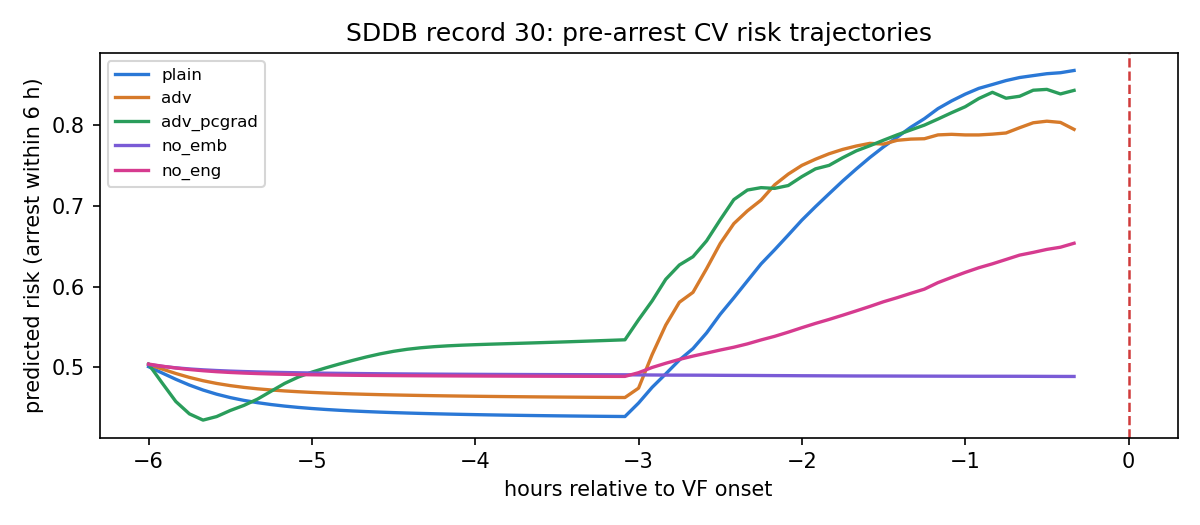
\includegraphics[width=\linewidth]{fig05_sddb_trajectory.png}
\caption{Cross validated risk trajectories for one real patient, hours relative
to ventricular fibrillation onset. The predicted risk does not rise before the
real event in any variant.}
\end{figure}

\begin{figure}[h]
\centering
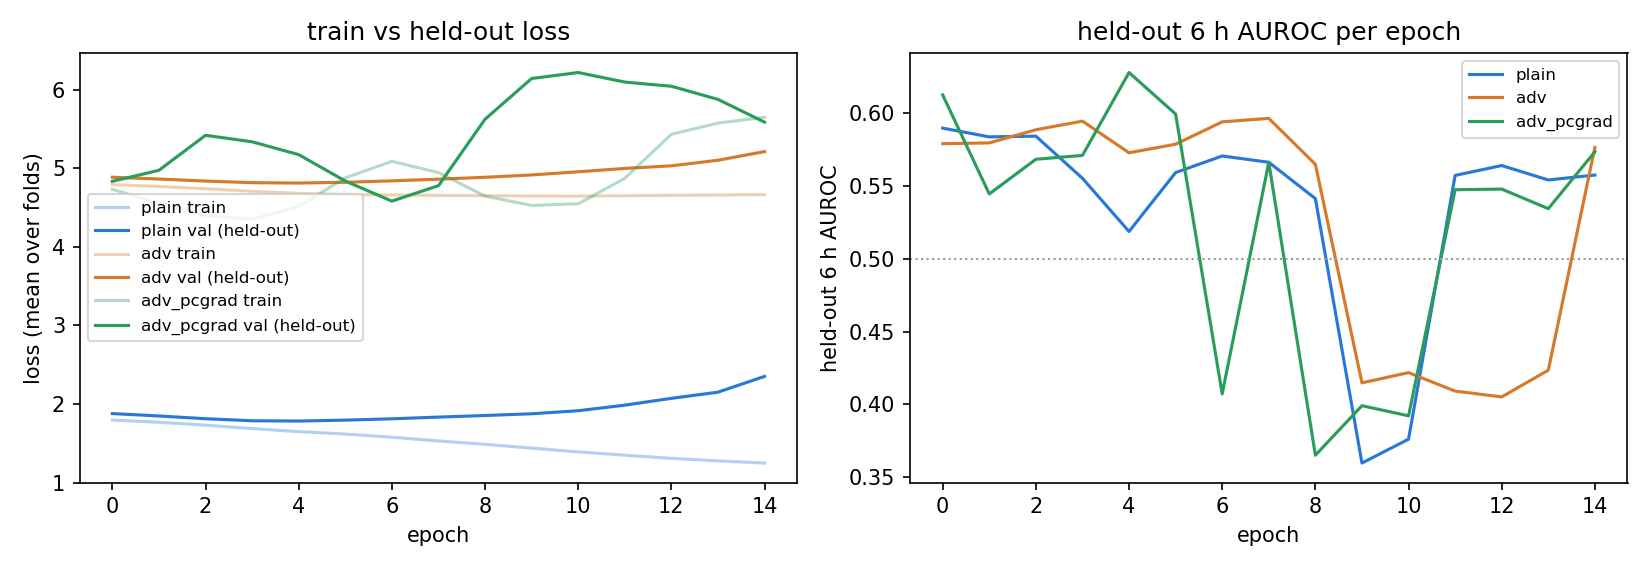
\includegraphics[width=\linewidth]{fig06_sddb_curves.png}
\caption{Train versus held out loss per epoch (mean over folds) for the three
identity adversarial variants, and held out 6 hour AUROC per epoch.}
\end{figure}

\begin{figure}[h]
\centering
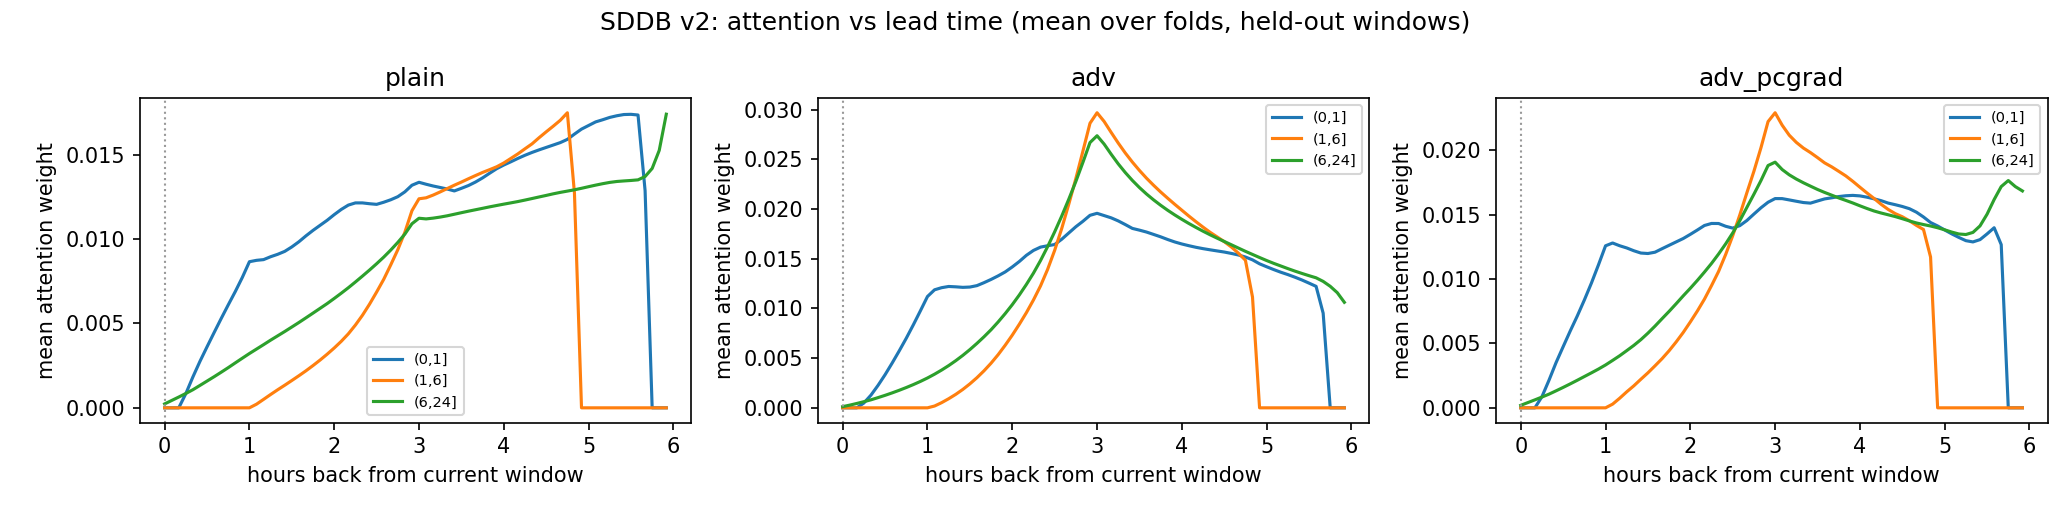
\includegraphics[width=\linewidth]{fig07_sddb_attention.png}
\caption{Attention salience by lead time bin (mean over folds): the model
spreads attention over history and puts near zero weight on the current
window.}
\end{figure}

\section{Slow risk layer}
QT interval, T wave alternans index, QRS width and long term heart rate
variability markers are aggregated over 3 hour blocks and scored with a
logistic regression (59 blocks, 16 records, grouped cross validation, 0.5 hour
label margin rule). The layer stays below chance on this data: 1 hour AUROC
0.426 [0.193, 0.667] with 5 positives, 6 hour AUROC 0.313 [0.190, 0.400] with
28 positives. Slow electrocardiogram markers alone do not separate pre arrest
blocks from far blocks on Holter recordings, consistent with the short horizon
result.

\begin{figure}[h]
\centering
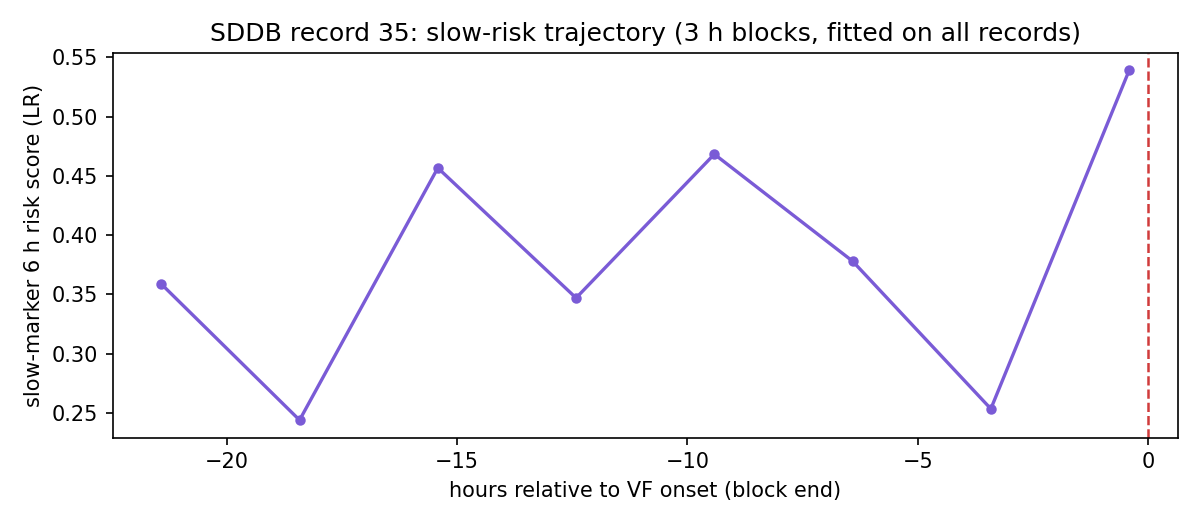
\includegraphics[width=\linewidth]{fig08_slow_risk_trajectory.png}
\caption{Slow risk score per 3 hour block for the record with the longest pre
arrest region (logistic regression fitted on all records, illustrative).
The score does not rise as the event approaches.}
\end{figure}

\section{Robustness}
Five perturbation families were applied to the held out replay patients and
scored with the three trained models (concat versus mask aware gate and
weight). Waveform perturbations were re embedded through the real encoders:
ECG noise at SNR 20, 10 and 5 dB, baseline wander, 50 Hz mains, flatline
halves, saturation, and PPG noise at 5 dB. Feature level stress covered
vitals noise at 0.5 to 2 times the per column standard deviation, missing
PPG, delayed measurements shifting the whole vector by 5, 10 and 15 minutes,
and a sensor failure where PPG dies mid stay.

\begin{table}[h]
\centering
\caption{6 h AUROC under perturbation (clean baseline 0.929 to 0.945).}
\begin{tabular}{lccc}
\toprule
Perturbation & concat & gate & weight \\
\midrule
Missing PPG & 0.937 & 0.952 & 0.947 \\
Delay 5 min & 0.926 & 0.943 & 0.941 \\
Delay 10 min & 0.923 & 0.942 & 0.940 \\
Delay 15 min & 0.920 & 0.941 & 0.938 \\
Sensor failure (PPG dies mid stay) & 0.929 & 0.945 & 0.943 \\
Vitals noise 2x std & 0.929 & 0.951 & 0.943 \\
ECG noise 5 dB & 0.934 & 0.949 & 0.945 \\
ECG flatline halves & 0.928 & 0.940 & 0.952 \\
ECG saturation & 0.929 & 0.946 & 0.943 \\
PPG noise 5 dB & 0.958 & 0.949 & 0.963 \\
\bottomrule
\end{tabular}
\end{table}

Every perturbation lands within 0.03 of clean. The only directional effect
is the delay family, which degrades monotonically but mildly (concat 0.929 to
0.920 at 15 minutes). Missing PPG, sensor failure, vitals noise and all ECG
artifacts leave the score unchanged, and the mask aware models behave like
concat here because synthetic PPG carries little signal.

Honest caveats: this measures robustness on synthetic data, where the risk
signal lives in the vitals and engineered blocks (the earlier ablation
finding), so waveform robustness partly reflects the encoders and partly that
the embeddings matter little there; the quality gates would reject flatline
and saturation windows in the real pipeline, and these tests bypassed the
gates and still held; and with 2 replay patients these are point estimates.

\begin{figure}[h]
\centering
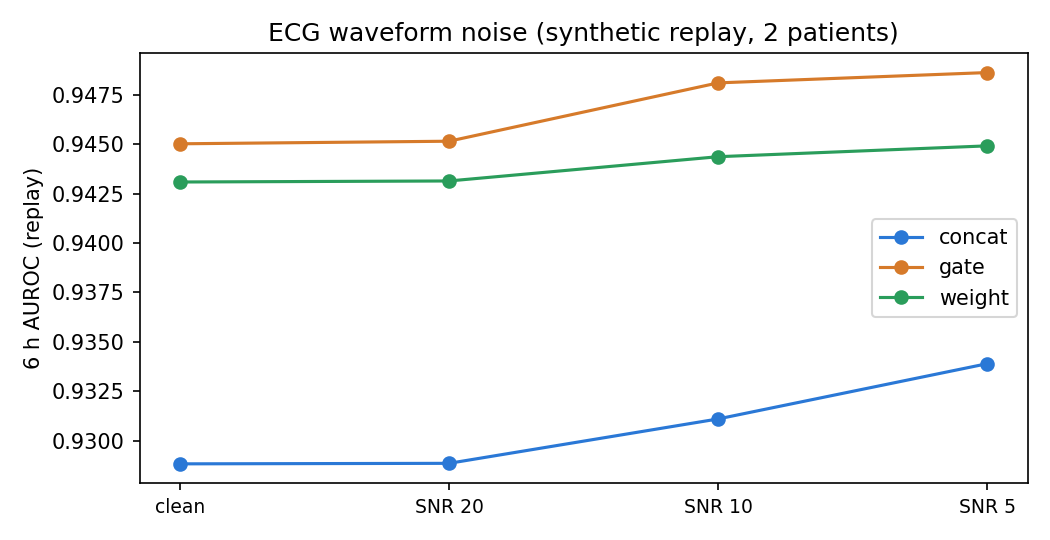
\includegraphics[width=\linewidth]{fig09_robustness_noise.png}
\caption{6 h AUROC versus ECG waveform noise level (synthetic replay). No
degradation down to SNR 5 dB.}
\end{figure}

\begin{figure}[h]
\centering
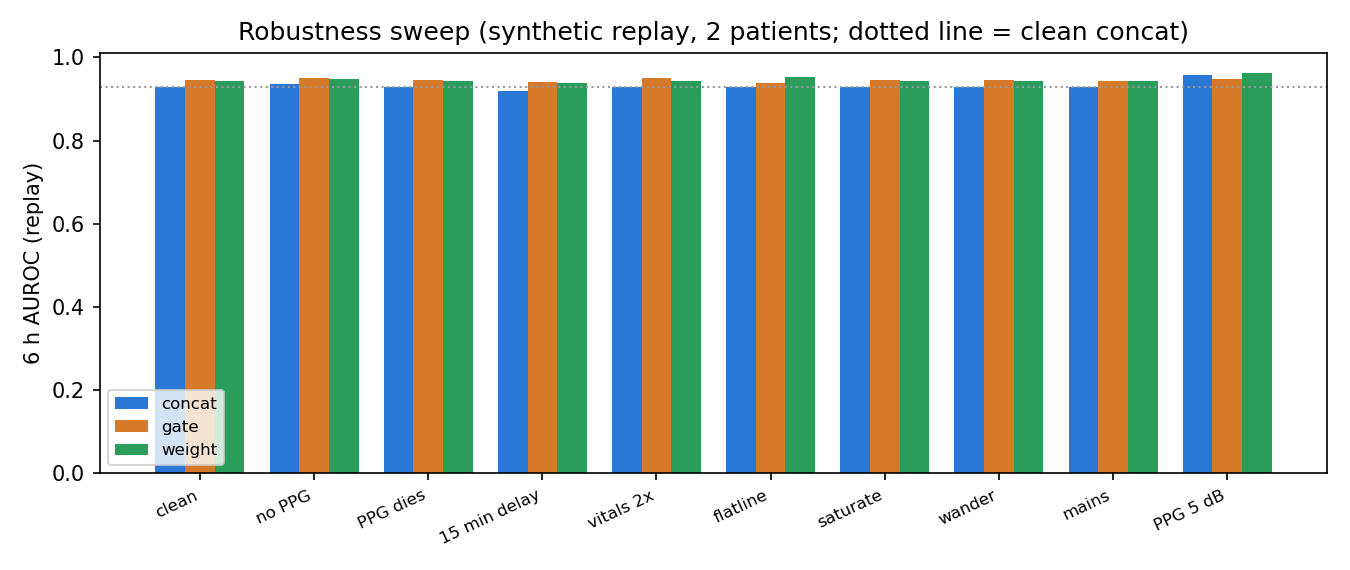
\includegraphics[width=\linewidth]{fig10_robustness_failure.png}
\caption{Robustness sweep across all perturbation families (synthetic replay;
the dotted line is the clean concat score).}
\end{figure}

\section{Summary of findings}
The pipeline machinery is validated end to end on synthetic data. The
synthetic trained model carries nothing to real electrocardiograms (zero shot
at chance). No model variant trained on 20 real patients beats chance at 6
hours. At 1 hour a weak signal exists and comes from engineered rate features,
not from the foundation model embeddings. The decisive next step is the
credentialed MIMIC III evaluation with full modalities.

\end{document}